\documentclass[12pt]{standalone}

\input{../../tikzpic_packages.tex}


\begin{document}
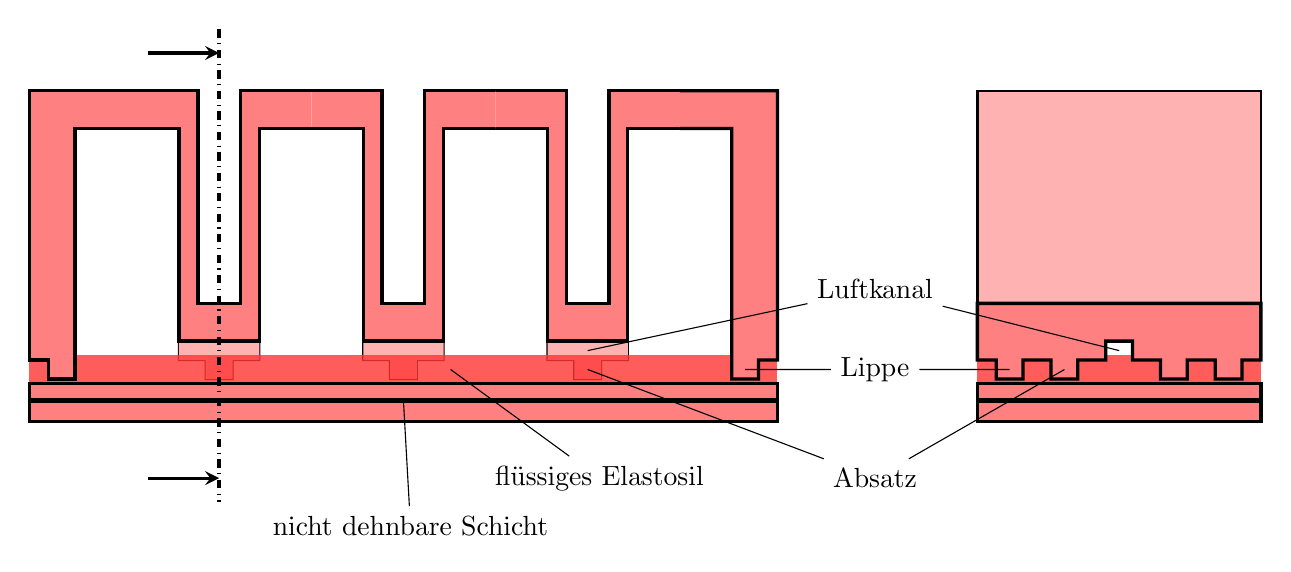
\begin{tikzpicture}[scale=.6,
kontur/.style={black, very thick},
konturback/.style={thick},
elastosil/.style={fill=red!50},	% geschnittenes Elastosil
elaback/.style={fill=red!30},	% Elastosil im Hintergrund
flussig/.style={fill=red!80, opacity=.8},	% flüssiges Elastosil
nichtdehnbar/.style={fill=black},	% Papierstreifen 
schrift/.style={black, thin}
]

%%%%%%%%%%%%%%%%%%%%%%%%%%%%%%%%%%%%%%%%5


% Defs of Basis

\def\hy{4.5}		% Höhe y
\def\hx{1.3}		% Halbe Höhe x
\def\xl{1.3}		% x distance luecke
\def\thick{.2}	% Halbe Dicke
\def\hya{.4}	% Höhe y Absatz
\def\hyl{.8}	% Höhe Luftkanal		
\def\N{4}		% Anzahl Kammern

% Defs of Bottom

\def\bhy{.8}		% Höhe Boden
\def\bdy{.1}		% Abstand zwischen Basis und Boden
\def\fhy{.6}		% Höhe ElastosilLevel


% Defs of Schnitt

\def\xshift{18}
\def\sxges{6}


% Implicite
\pgfmathsetmacro{\xges}{\hx+\hx+\xl}
\pgfmathsetmacro{\xgesh}{\xges/2}
\pgfmathsetmacro{\yges}{\hy+\hyl}
\pgfmathsetmacro{\hxa}{(\xl+\thick+\thick)/3}
\pgfmathsetmacro{\X}{\xges*(\N-2)}
\pgfmathsetmacro{\Xges}{\X+\xges+2*\thick+2*\hxa+2*\hx}
\pgfmathsetmacro{\bhyh}{\bhy/2}
\pgfmathsetmacro{\shx}{1/4*(\sxges-5*\hxa-4*\thick)}





%%%%%%%%%%%%%%% BASIS %%%%%%%%%%%%%%%%%%

\foreach \x[count=\i] in {0, \xges, ..., \X}{

\path (\x,0)coordinate(OL); 	% Koord oeben links
\path (OL)++(\xges,-\thick-\thick-\thick)coordinate(B);
\def\konturOben{
(OL)++(0,\thick)--++(\hx+\thick,0)--++(0,-\hy)--++(\xl-\thick-\thick,0)--++(0,\hy)--++(\hx+\thick,0)coordinate(OR)
}
\def\konturUnten{
(B)
--++(-\hx+\thick,0)
--++(0,-\hy)coordinate(UR)
--++(-\xl-\thick-\thick,0)coordinate(UL)coordinate[midway](Luftkanal\i)
--++(0,\hy)
--++(-\hx+\thick,0)
}
\def\konturBack{
(UL)
--++(0,-\hyl+\hya)
--++(\hxa,0)
--++(0,-\hya)
--++(\hxa,0)coordinate[midway](Absatz\i)
--++(0,\hya)
--++(\hxa,0)--(UR)}

\path \konturUnten; % Just for defining the nodes



%% Elastosil
\draw[konturback] \konturBack;
\path[elaback] \konturBack;

\path[elastosil] \konturOben -- \konturUnten;
\draw[kontur] \konturOben;
\draw[kontur] \konturUnten;

}

%%%%%%%%%%%%%%% FlUEssig %%%%%%%%%%%%%%%%%%

\path[flussig] (-\hx-\thick-\hxa,-\yges-\bdy-\thick-\thick-\thick) rectangle ++(\Xges,\fhy)coordinate[midway](Flussig);


%% Enden
\def\konturEndeRechts{
(B)
--++(\hx-\thick,0)
--++(0,-\yges)
--++(\hxa,0)coordinate[midway](Lippe)
--++(0,\hya)
--++(\thick+\thick,0)
--++(0,\yges-\hya+\thick+\thick+\thick+\thick)--(OR)}
\path[elastosil] \konturEndeRechts;
\draw[kontur] \konturEndeRechts;


\def\konturEndeLinks{
(0,-\thick-\thick-\thick)--++(-\hx+\thick,0)--++(0,-\yges)--++(-\hxa,0)coordinate(help)--++(0,\hya)--++(-\thick-\thick,0)--++(0,\yges+\hya)--(0,\thick)}
\path[elastosil] \konturEndeLinks;
\draw[kontur] \konturEndeLinks;

\path (help)++(-\thick-\thick,-\bdy)coordinate(BOL);


%%%%%%%%%%%%%% Boden %%%%%%%%%%%%%%%%%%%%%%%%%%

\path[elastosil] (BOL)--++(\Xges,0)--++(0,-\bhy)coordinate(BUR)--++(-\Xges,0)--cycle;
\draw[kontur] (BOL)rectangle(BUR);
\path[nichtdehnbar] (BUR)++(0,\bhyh)rectangle++(-\Xges,.1)coordinate[midway](nichtDehnbar);






%%%%%%%%%%%%%%%%%%%%%%%%% SCHNITT ANSICHT %%%%%%%%%%%%%%%%%%%%%%%%



\def\konturSchnitt{
(\xshift,-\yges-\thick-\thick-\thick+\hya)coordinate(SUL)
--++(\thick+\thick,0)
--++(0,-\hya)
--++(\hxa,0)coordinate[midway](LippeSchnitt)
--++(0,\hya)
--++(\shx,0)
--++(0,-\hya)
--++(\hxa,0)coordinate[midway](AbsatzSchnitt)
--++(0,\hya)
--++(\shx,0)
--++(0,\hyl-\hya)
--++(\hxa,0)coordinate[midway](LuftkanalSchnitt)
--++(0,-\hyl+\hya)
--++(\shx,0)
--++(0,-\hya)
--++(\hxa,0)
--++(0,\hya)
--++(\shx,0)
--++(0,-\hya)
--++(\hxa,0)
--++(0,\hya)
--++(\thick+\thick,0)
--++(0,\hyl-\hya+\thick+\thick+\thick+\thick)
--++(-\sxges,0) coordinate(help)
--cycle}

\path \konturSchnitt;
\path (SUL)++(0,-\hya-\bdy)coordinate(BOR);

\path[flussig] (BOR) rectangle ++(\sxges,\fhy);
\path[elastosil] \konturSchnitt;
\path[elaback] (help)rectangle++(\sxges,\hy);
\draw[konturback] (help)rectangle++(\sxges,\hy);
\draw[kontur] \konturSchnitt;

\path[elastosil] (SUL)++(0,-\hya-\bdy)rectangle++(\sxges,-\bhy);
\path[nichtdehnbar] (SUL)++(0,-\hya-\bdy-\bhyh)rectangle++(\sxges,.1);
\draw[kontur] (SUL)++(0,-\hya-\bdy)rectangle++(\sxges,-\bhy);



%% Schnitt
\draw [dashdotted, very thick] (\xgesh,1.5) --++(0,-10);
\draw [-stealth, very thick] (\xgesh-1.5,-8)--++(1.5,0);
\draw [-stealth, very thick] (\xgesh-1.5,1)--++(1.5,0);



%%%%%%%%%%%%%%%%%%%%%%%%% BESCHRIFTUNG %%%%%%%%%%%%%%%%%%%%%%%%

\path (\Xges,-5.7)node[](LippeText){Lippe};
\draw[schrift] (LippeSchnitt)++(0,.2)--(LippeText);
\draw[schrift] (Lippe)++(0,.2)--(LippeText);


\path (\Xges,-8)node(AbsatzText){Absatz};
\draw[schrift] (AbsatzSchnitt)++(0,.2)--(AbsatzText);
\draw[schrift] (Absatz3)++(0,.2)--(AbsatzText);

\path (\Xges,-4)node(LuftkanalText){Luftkanal};
\draw[schrift] (LuftkanalSchnitt)++(0,-.2)--(LuftkanalText);
\draw[schrift] (Luftkanal3)++(0,-.2)--(LuftkanalText);


\path (6,-9) node(DehnbarText){nicht dehnbare Schicht};
\draw[schrift] (nichtDehnbar)++(0,0)--(DehnbarText);

\path (10,-8) node(FlussigText){flüssiges Elastosil};
\draw[schrift] (Flussig)++(1,0)--(FlussigText);


\end{tikzpicture}
\end{document}